\section{Introduction}

\subsection{The Problem Of Units}

Units are everywhere. We encounter units and quantity expressions in everyday life wherever we go. When driving on the road we see a speed limits on signs (for example $30 \frac{\text{km}}{h}$). When we go shopping there are different shoe sizes. When we buy something, we pay a currency of $30 \text{\euro}$. Everything is being quantified. This is also the case in science papers. Many, if not all, papers have 1 or more quantity expressions in them. Approximatly 1\% of all letters in scienficic papers belong to a quantity expression\ednote{Verify this}.

This in itself is not a problem. The problem occurs when different units are used to describe the same quantity. In most of the world, the metric system is used to describe most quantities. Some countries still use non-SI units. These different units sometimes make it very difficult to talk about Quantities.

One notable example for this is the \textit{Mars Climate Orbiter} which was destroyed in 1999 when it entered the atmosphere of Mars because it received the non-standard units of \textit{pound-seconds} instead of the expected \textit{newton-seconds}\cite{nasa:mcor}.

\subsection{State Of The Art: Unit Converters And The SI System}

Out of convenience new units ones are constantly being invented. Hence there are many hundred units that already exist. Just converting between them is easy, googleing ``unit converter'' reveals about 12000000 results. Even Google itself has implemented a unit converter into its search engine.

However, all of these tools have a problem. They only convert units directly, meaning they require the user to enter the original units and desired units. This reuires the user to identity that there is a problem with units in the first place.

There is no tool which directly incorperates this translation of units into search results. Such a tool should find quantities independently of which units they are expressed in. It would make search efforts much easier, as fewer user input is required. It would no longer be required for the user to recognise that there is a problem.

In addition to this problem unit converters are usually very restricted in the units they support. They commonly store translation formulae for any pair of units to convert between. Hence they are difficult to extend with new units.

Their superficial handling of units usually does not take the underlying meaning, the semantics, into accoun On the other hand, The SI specification \cite{sispec} provides a very good insight into how units can be handled. It is precisely defined what each unit means and what kind of quantities can be expressed. It is a very formal approach. This approach does not take into account that it is sometimes less practical to user general units instead of specfic ones.

Neither this very formal nor the previous approach with unit converters can be efficiently used to solve the problem.

\subsection{Our Approach: A Semantic Quantity Expression Search}

That is why we want to build a search engine that unifies these approaches. It should be capable to find occurrences of quantity expressions within documents, no matter of their representation. For this we need several components: (1) an extensible system flexible enough to convert between units when needed, (2) a so-called spotter that finds occurrences of quantity expressions within documents, (3) a search algorithm that can take a quantity expression from the user and find equivalent quantities in the results from the spotter and (4) a front-end that allows the user to enter a quantity expression and receive the results.

For (1) we want to use a meta-mathematical theories approach which is implemented by a software called MMT. With the help of MMT this allows us to build an extendible unit system. This uses a concept of a theory graph in which units are related via so-called views and imports. These can be used to translate between them. Additionally, we can define a new unit and easily link it to any of the ones which have been defined previously. Point (2) will be taken on by Stiv Sherko in a seperate effort \cite{thesis:sharko}. The spotter finds quantity expressions inside documents which can almost directly be used by our system. For our search algorithm (3) we use a simple trick: We normalise spotted units. A normal form is then used to efficiently index the harvest delivered from the previous step. Finally for (4) we built a frontend which allows the user to enter quantity expressions. It is deployed at \cite{self:sqesdemo}. A basic sketch of the system can be found in Figure \ref{fig:system}.

\begin{figure}[h]
  \begin{center}
    
  \usetikzlibrary{fit,arrows,calc,positioning}
  \tikzstyle{comp} = [rectangle, draw, node distance=3cm, text width=6em, text centered, rounded corners, minimum height=4em, thick]
  \tikzstyle{compB} = [comp, fill=blue!20]
  \tikzstyle{compF} = [comp, fill=yellow!20]
  \tikzstyle{inter} = [draw, -latex',thick]

  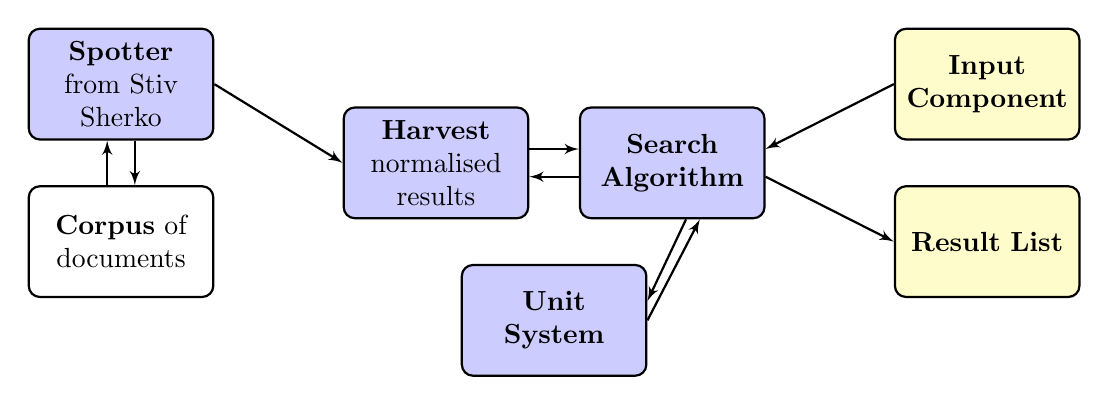
\begin{tikzpicture}[auto]
      \node [comp] (Q) at (-4, -1) {
        \textbf{Corpus} of documents
      };

      \node [compB] (S) at (-4, 1) {
        \textbf{Spotter} from Stiv Sherko
      };

      \draw [inter] ([xshift=-5pt] Q.north) -- ([xshift=-5pt] S.south);
      \draw [inter] ([xshift=5pt] S.south) -- ([xshift=5pt] Q.north);

      \node [compB] (H) at (0, 0) {
        \textbf{Harvest} normalised results
      };

      \draw [inter] (S.east) -- (H.west);

      \node [compB] (SA) at (3, 0) {
        \textbf{Search Algorithm}
      };

      \draw [inter] ([yshift=5pt] H.east) -- ([yshift=5pt] SA.west);
      \draw [inter] ([yshift=-5pt] SA.west) -- ([yshift=-5pt] H.east);

      \node [compF] (R) at (7, -1) {
        \textbf{Result List}
      };

      \draw [inter] ([yshift=-5pt] SA.east) -- (R.west);

      \node [compF] (Q) at (7, 1) {
        \textbf{Input Component}
      };

      \draw [inter] (Q.west) -- ([yshift=5pt] SA.east);

      \node [compB] (US) at (1.5, -2) {
        \textbf{Unit System}
      };

      \draw [inter] (US.east) -- ([xshift=10pt] SA.south);
      \draw [inter] ([xshift=5pt] SA.south) -- ([yshift=7pt] US.east);

  \end{tikzpicture}

  \end{center}

  \caption{Basic Architecture Of The System. Components Of The Backend Are Drawn In Blue, Components Of The Frontend In Yellow. }
  \label{fig:system}
\end{figure}


\subsection{Overview}

This thesis is organised as follows: In section \ref{sec:mathoverview} we start by giving an introduction to mathematical theory modeling. We proceed in section \ref{sec:strucqe} to talk about how quantity expressions can be formalised and in section \ref{sec:mqes} we apply these insights in order to start building in our search engine. In section \ref{sec:pit} we present the implementation in detail by describing how a search query is processed and how it is presented to the end user. We finally conclude with discussing the limits of this implementation as well as future work in section \ref{sec:future}.
